\chapter{Image Compression}

A data compression algorithm transforms the data to occupy a less space. The original data is encoded by a program called encoder, to a compressed representation using a fewer number of bits. Decoder is responsible for decompressing the compressed representation. 

\begin{figure}[!ht]
    \centering
    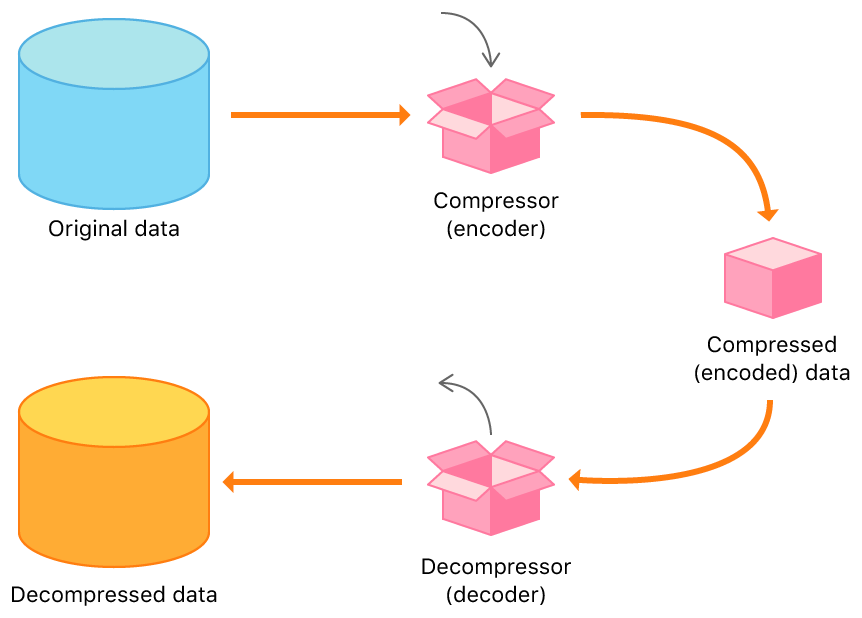
\includegraphics[width=0.50\textwidth]{fig/2-1.png}
    \captionsource{Compression phases}
    {\url{https://developer.apple.com/documentation/compression}}
    \label{fig:phasesCompression}
\end{figure}

Image compression is very crucial in order to reduce the size of disk space used as well as reduce the amount of internet bandwidth used while loading images. It’s also important to compress images for people accessing the internet via low bandwidth connections.

\section{Lossy vs. Lossless}

The compression technique where the decompressed data is exactly same as original data is called as lossless compression otherwise it is known as lossy compression technique because some information is lost during coding-encoding phase. Two well-known codecs for image compression are JPEG and PNG. PNG is lossless and JPEG is lossy.

\vspace{2em}

\begingroup
\centering
    \begin{tabular}{ | p{7cm} | p{7cm} | }
    \hline
    Lossy & Lossless \\ \hline
    A compression
    that permits reconstruction only of an approximation of the original data, though usually with an improved compression rate. & A class of data compression that allows the original data to be perfectly reconstructed from the compressed data. \\ \hline
    Reduces the quality. & Does not reduce the quality. \\ \hline
    Data reduction is higher. & Data reduction is lower. \\ \hline
    Commonly used to compress multimedia data such as audio (MP3), video and image (JPEG) files. & Used commonly for text, data files, etc. \\
    \hline
    \end{tabular}
\captionof{table}{Lossy vs Lossless}\label{tbl:lossyvslossless}
\endgroup


\section{Dimensionality Reduction PCA}

Principal components analysis (PCA) is one of a family of techniques for taking high-dimensional data, and using the dependencies between the variables to represent it in a more tractable, lower-dimensional form, without losing too much information. PCA is one of the simplest and most robust ways of doing such dimensionality reduction.

PCA is mathematically defined as an orthogonal linear transformation that transforms the data to a new coordinate system such that the greatest variance by some scalar projection of the data comes to lie on the first coordinate (called the first principal component), the second greatest variance on the second coordinate, and so on.


\begin{figure}[!ht]
    \centering
    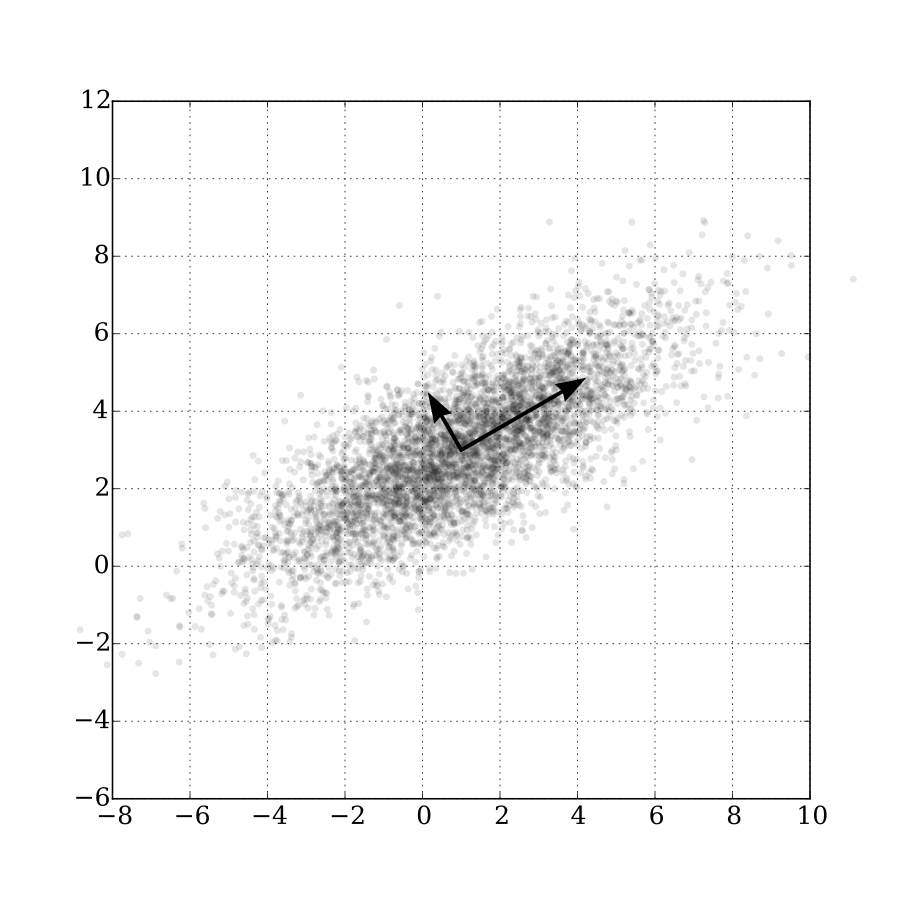
\includegraphics[width=0.65\textwidth]{fig/2-2.png}
    \captionsource{PCA of a multivariate Gaussian distribution centered at (1,3) with a standard deviation of 3 in roughly the (0.866, 0.5) direction and of 1 in the orthogonal direction.}
    {\url{https://en.wikipedia.org/wiki/Principal_component_analysis}}
    \label{fig:phasesCompression}
\end{figure}


Let $W$ be a $d \times d$ matrix whose columns are the principal components of $X$. The transformation $T = X W$ maps a data vector $x_{(i)}$ from an original space of $d$ variables to a new space of $d$ variables which are uncorrelated over the dataset. However, not all the principal components need to be kept. Keeping only the first $L$ principal components, produced by using only the first $L$ eigenvectors, gives the truncated transformation:

$T_L = XW_L$


where the matrix $T_L$ now has $n$ rows but only $L$ columns. In other words, PCA learns a linear transformation 
$t = W^{T}x, x \in \Re^{d}, t \in \Re^{L}$, where the columns of $d \times L$ matrix $W$ form an orthogonal basis for the $L$ features (the components of representation t) that are decorrelated. By construction, of all the transformed data matrices with only $L$ columns, this score matrix maximises the variance in the original data that has been preserved, while minimising the total squared reconstruction error $\left \| TW^T - T_LW_L^T\right \|_2^2 or \left \| X - X_L \right \|_2^2$.

The basic steps for computing the PCA is as follows:

\begin{enumerate}
    \item Standardize the d-dimensional dataset.
    \item Construct the covariance matrix.
    \item Decompose the covariance matrix into its eigenvectors and eigenvalues.
    \item Sort the eigenvalues by decreasing order to rank the corresponding eigenvectors.
    \item Select $L$ eigenvectors which correspond to the $L$ largest eigenvalues, where $L$ is the dimensionality of the new feature subspace $L \leq d$.
    \item Construct a projection matrix $W_L$ from the "top" $L$ eigenvectors.
    \item Transform the $d$-dimensional input dataset $X$ using the projection matrix $W_L$ to obtain the new $L$-dimensional feature subspace.
\end{enumerate}

\vspace{1em}

\begin{figure}[!ht]
    \centering
    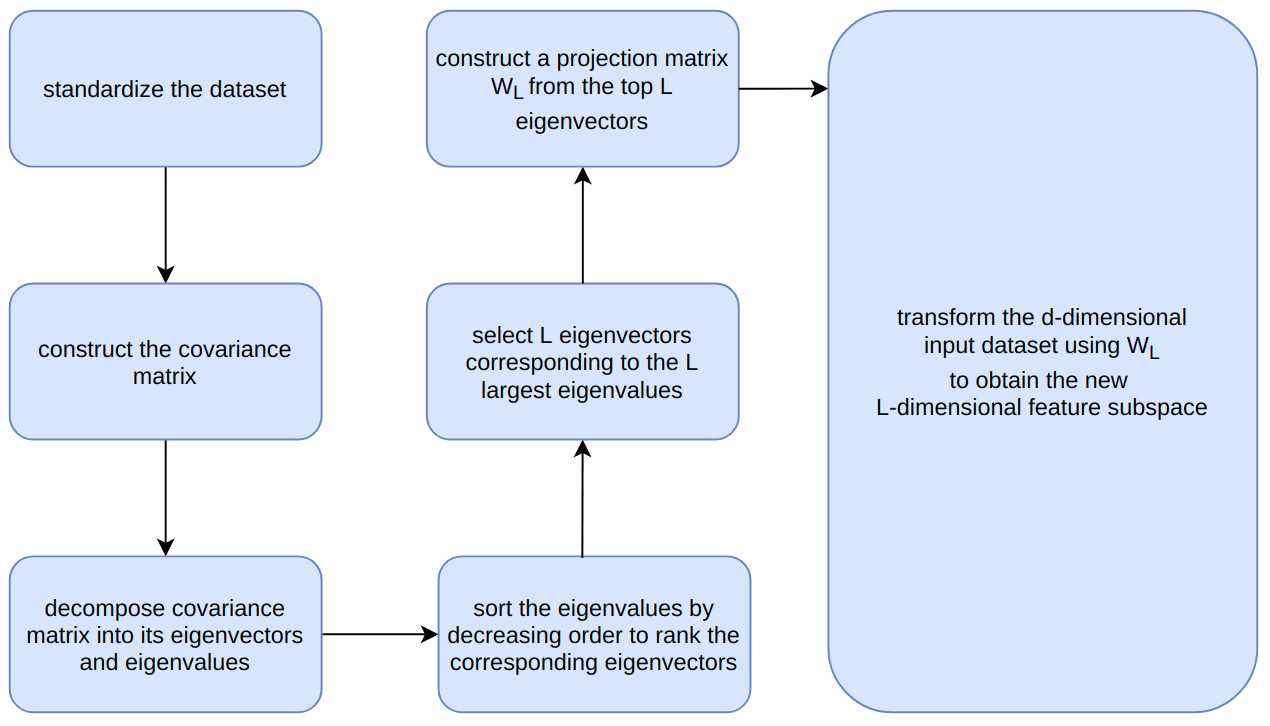
\includegraphics[width=0.75\textwidth]{fig/2-3.png}
    \caption{Steps for dimensionality reduction using PCA}
    \label{fig:dimensionalityReductionSteps}
\end{figure}

\vspace{1em}

\section{Image compression using PCA}

We will follow the steps mentioned in the previous section for dimensionality reduction using PCA. The results of the experiments are tabulated below:

\begin{figure}[!ht]
    \centering
    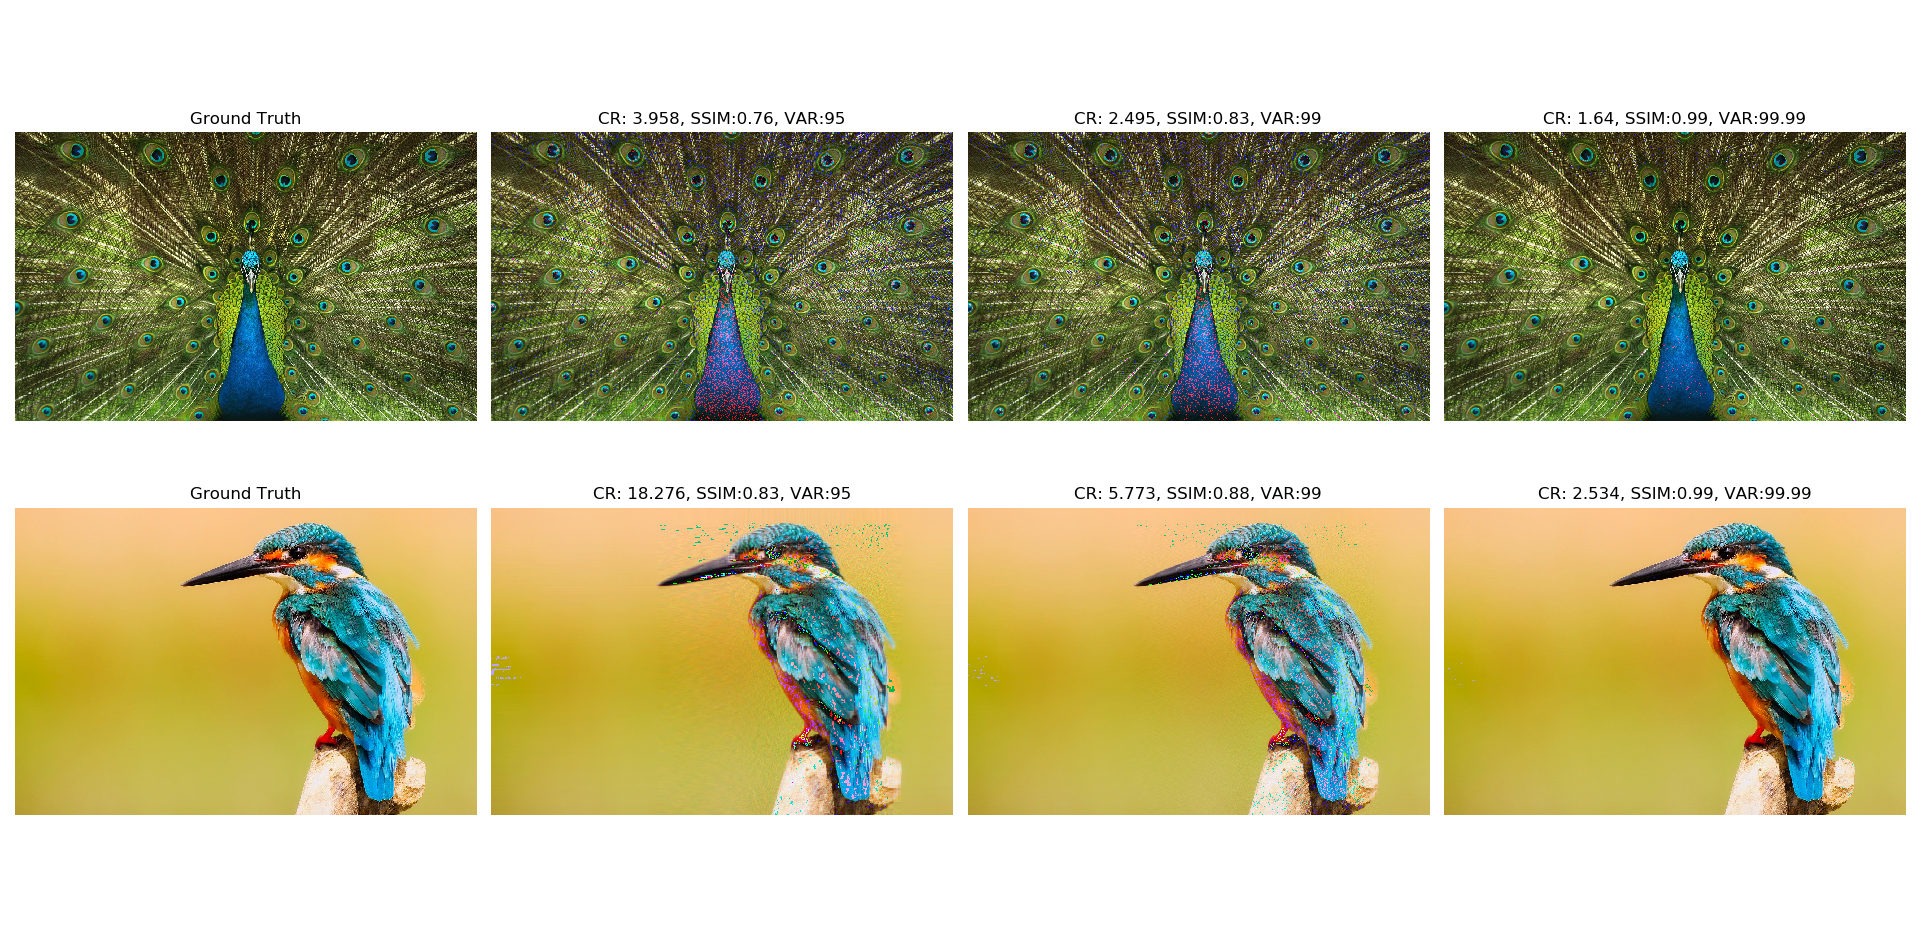
\includegraphics[width=1\textwidth]{fig/2-4.png}
    \caption{ CR = Compression Ratio, SSIM = Structural Similarity Index, VAR = Variance. Results of compression using the PCA method. Higher variance leads to more number of principal components and higher is the reconstructed image quality and lower the compression rate.}
    \label{fig:imageCompressionUsingPCA}
\end{figure}

Code for the above test can be found here: \href{https://github.com/KishoreKaushal/ImageCompression/tree/master/PCA}{@KishoreKaushal/ImageCompression/}

It is clear from the above experiment that higher variance leads to more number of principal components and higher is the reconstructed image quality and lower the compression rate. Infact, the first $L$ principal components is selected to get atleast the given number of variance.